\documentclass[conference]{IEEEtran}
\usepackage[T1]{fontenc}
\usepackage{graphicx}
\usepackage{booktabs}
\usepackage{listings}
\usepackage{xcolor}
\usepackage{url}
\usepackage[hidelinks]{hyperref}
\graphicspath{{../docs/}}
\lstset{basicstyle=\ttfamily\scriptsize, breaklines=true, breakatwhitespace=false,
        columns=fullflexible, frame=single, framerule=0.3pt, rulecolor=\color{gray},
        xleftmargin=2pt, xrightmargin=2pt}
\newcommand{\code}[1]{\texttt{\small #1}}

\begin{document}

\title{A Multi-Pipeline ETL and Reporting Framework\\for NASA Web Server Logs: Phase~1 Design}

\author{\IEEEauthorblockN{Tushar (BT2024022) \quad Sahiti (BT2024163) \quad Aman (BT2024123) \quad Prajwal (BT2024245)}
\IEEEauthorblockA{\textit{DAS 839 NoSQL Systems, End-Semester Project, Phase 1 Review}}}

\maketitle

\begin{abstract}
We present the Phase~1 design of a tool that runs one fixed ETL and analytics workload over the
NASA Kennedy Space Center HTTP logs (July and August 1995) on a pipeline chosen by the user, and
loads the results into PostgreSQL for reporting. Two pipelines, MongoDB and Hive, are fully
implemented; Pig and MapReduce follow in Phase~2 on the same framework. All parsing and
aggregation run inside the selected engine. A shared set of machine-readable \emph{contracts}
(parsing regexes, output schemas, batching rules) keeps the engines equivalent, and a
row-by-row checker proves it: on all 3,461,613 records, Hive and MongoDB produce identical
results for every batch and for the whole run.
\end{abstract}

\section{Team and Work Division}
Two members built each Phase~1 engine; within each pair, one member took ingestion, parsing
and Q1, the other the harder queries Q2 and Q3. Each member also owns one shared component
(Table~\ref{tab:team}).

\begin{table}[h]
\caption{Work division}
\label{tab:team}
\centering
\small
\begin{tabular}{@{}p{0.2\columnwidth}p{0.74\columnwidth}@{}}
\toprule
Member & Work \\
\midrule
Tushar (A) & \textbf{MongoDB:} raw-line ingestion, parsing inside MongoDB, malformed records, Q1.
             \textbf{Shared:} controller, batcher, loader and CLI. \\
Sahiti (B) & \textbf{MongoDB:} Q2 and Q3.
             \textbf{Shared:} architecture, equivalence checker, database tests. \\
Aman (C)   & \textbf{Hive:} raw-line ingestion with RegexSerDe, parsing in HiveQL, malformed
             records, Q1. \textbf{Shared:} PostgreSQL reporting schema. \\
Prajwal (D)& \textbf{Hive:} Q2, Q3 and whole-run results. \textbf{Shared:} reporting module. \\
\midrule
All        & Shared contracts, Docker environment, benchmarks, Phase~1 review. \\
\bottomrule
\end{tabular}
\end{table}

\section{Problem and Requirements}
The input is the two unmodified NASA log files, 3,461,613 lines in Common Log Format. The tool
must parse each line into nine fields (host, timestamp, method, path, protocol, status, bytes,
plus derived date and hour), count malformed lines instead of dropping them, and compute three
queries: \textbf{Q1}~daily traffic per date and status code (requests, bytes); \textbf{Q2}~top~20
resources by requests, with bytes and distinct hosts; \textbf{Q3}~hourly errors (status
400--599): error count, total count, error rate and distinct error hosts. The input is
processed in batches of a user-chosen size, results are loaded into a relational database
with pipeline, run, batch and time of execution, and a reporting module displays them with the
run's metadata. Runtime is measured from the first byte read to the final database commit.

\section{Overall Design}
Fig.~\ref{fig:arch} shows the architecture. A Python \textbf{controller} (\code{python -m etl
run -{}-pipeline <p> -{}-batch-size <N>}) owns everything that must be identical across engines:
it creates the run, cuts batches, starts and stops the clock, checks record counts, and calls
one shared \textbf{loader}. Each engine implements a four-method interface
(\code{prepare}, \code{process\_batch}, \code{finalize}, \code{cleanup}) and writes four
result files per batch (\code{q1}, \code{q2}, \code{q3}, \code{malformed}) in PostgreSQL
\code{COPY} text format. Python never reads a log line: MongoDB and Hive do all parsing and
aggregation.

\begin{figure*}[t]
\centering
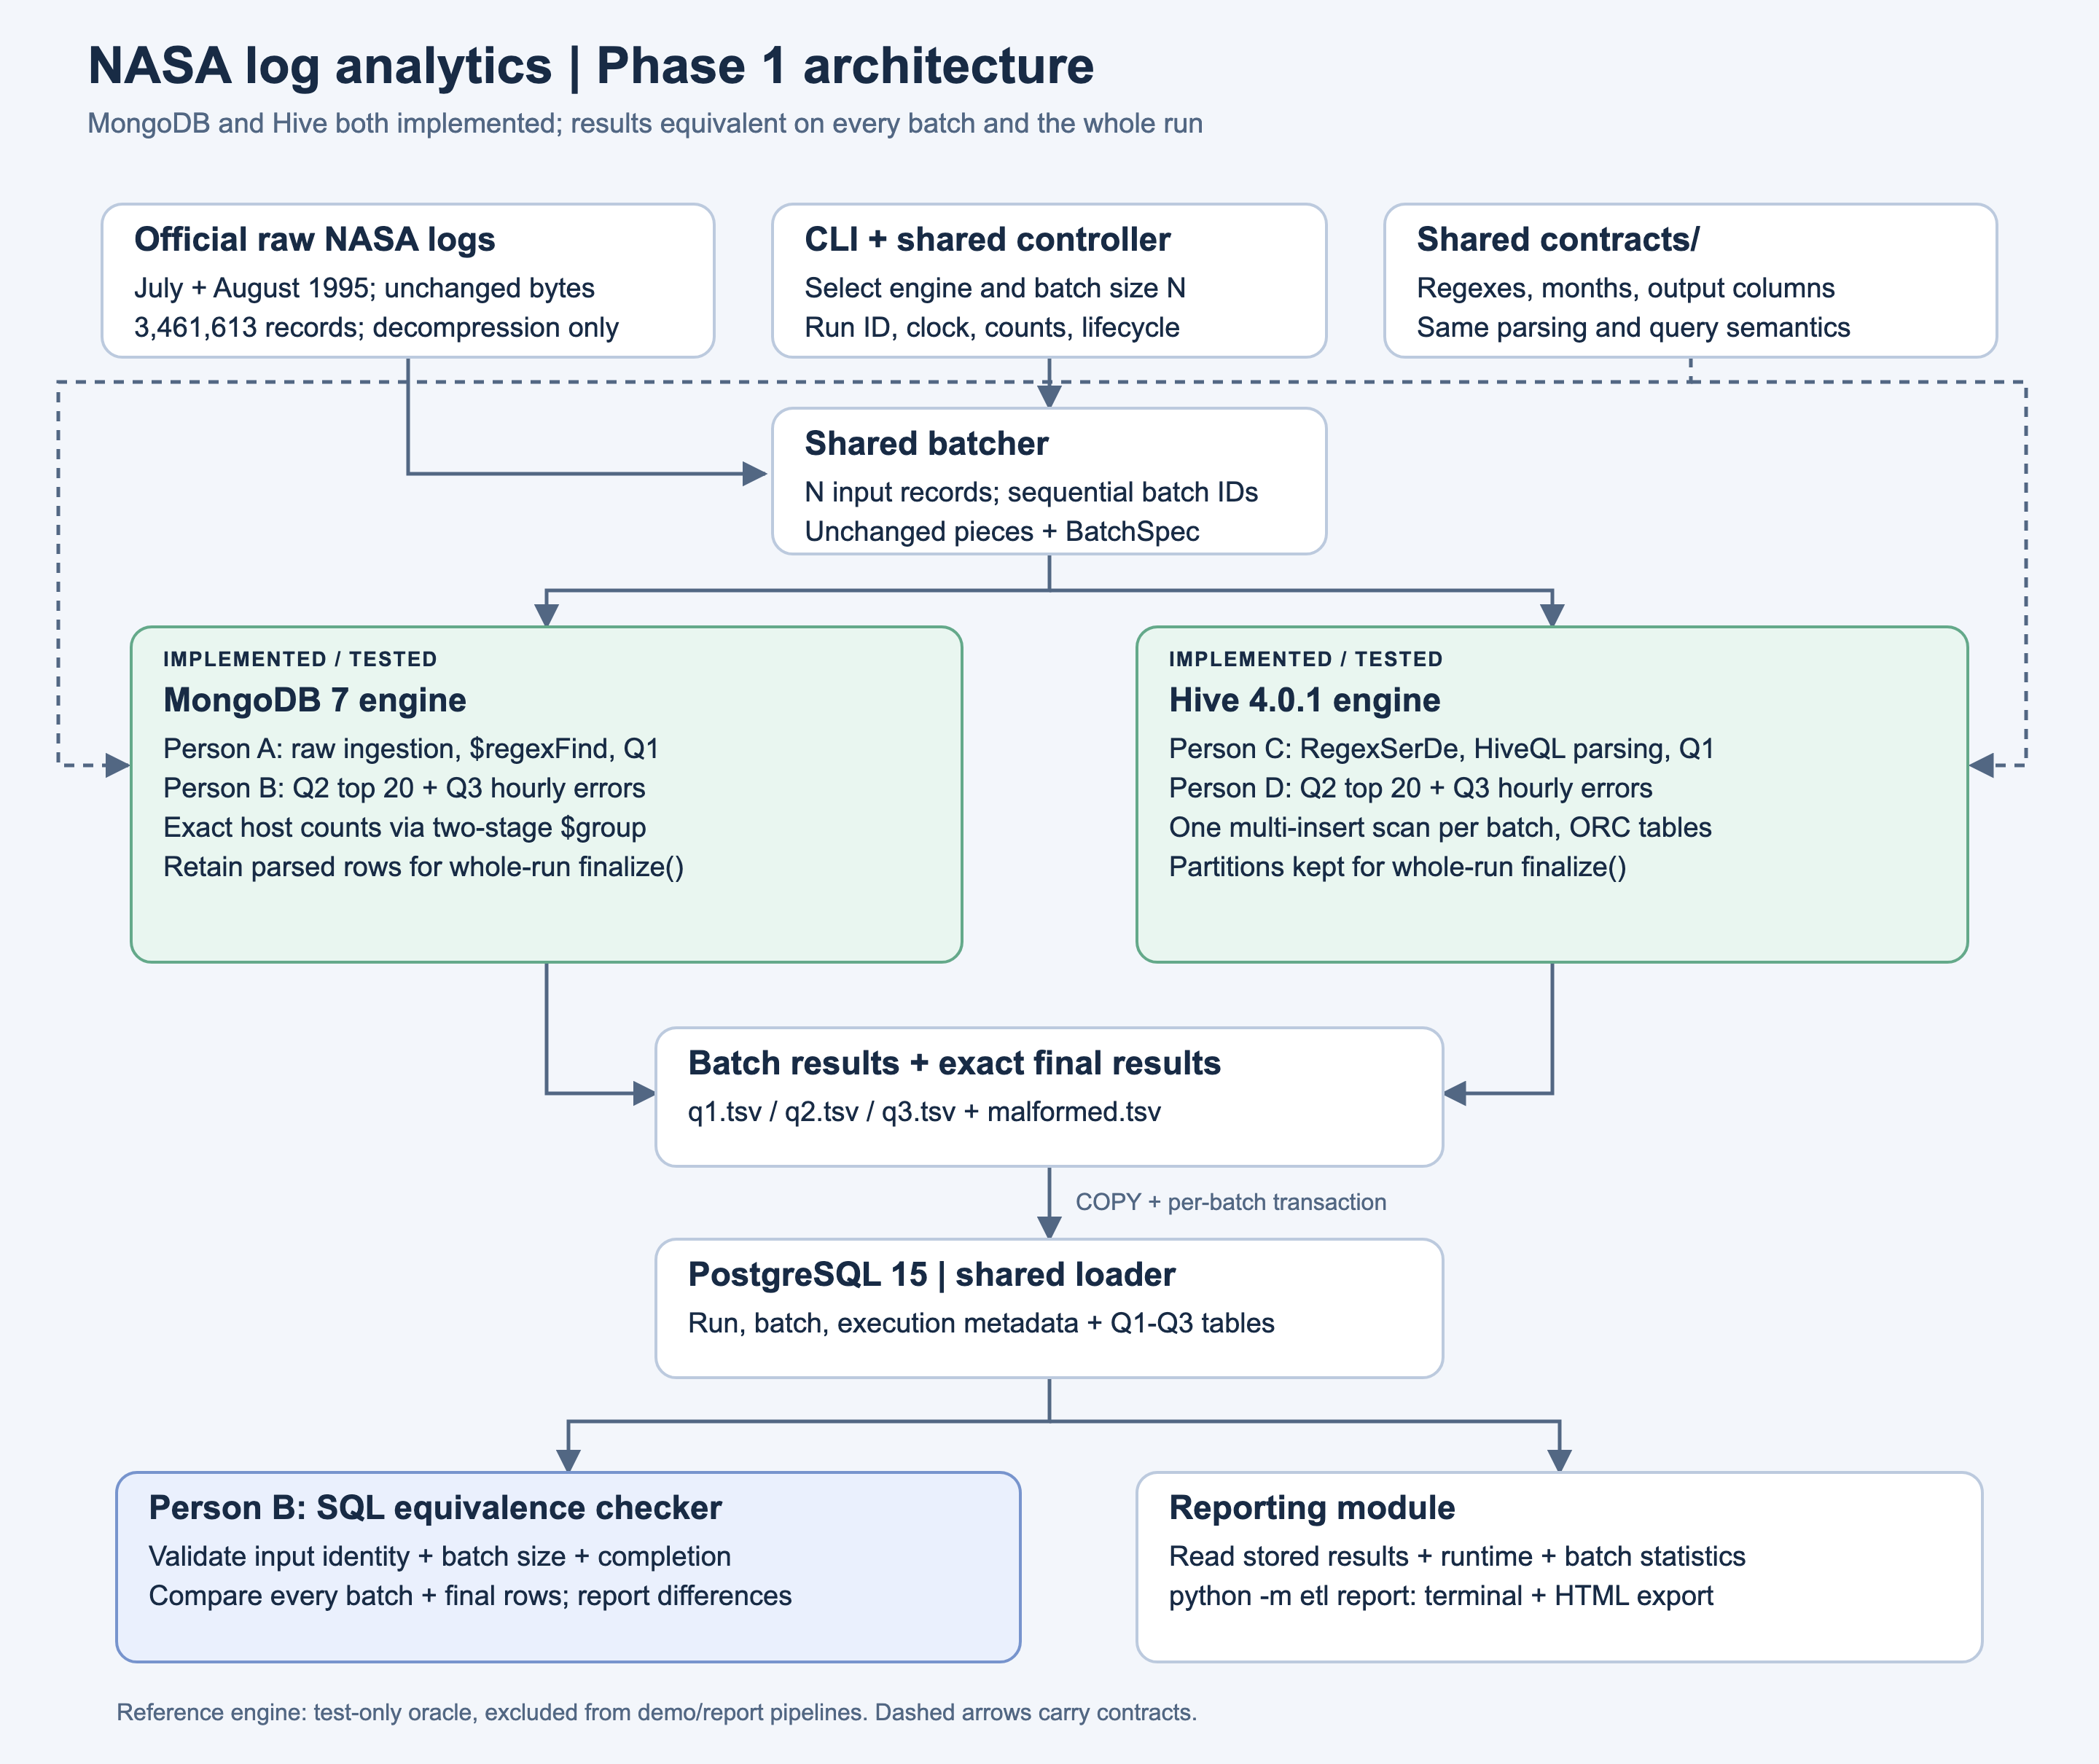
\includegraphics[width=0.78\textwidth]{architecture.png}
\caption{Phase 1 architecture. Dashed arrows carry the shared contracts.}
\label{fig:arch}
\end{figure*}

\textbf{Why MongoDB and Hive first.} They are the most different pair: a document store with
an aggregation framework versus SQL on Hadoop. If both agree under the same contracts, the
contracts are sound, and Pig and MapReduce become two more implementations of the same
interface.

\textbf{Environment.} PostgreSQL~15, MongoDB~7 and Hive~4.0.1 run in Docker with image
versions pinned by digest, so every member runs identical software on Windows and macOS.

\section{Parsing Strategy}
Every engine loads the same three regular expressions from \code{contracts/} at run time:

\begin{lstlisting}
envelope: ^([^ ]+) ([^ ]+) ([^ ]+) \[([0-9]{2})/([A-Za-z]{3})/([0-9]{4}):([0-9]{2}):([0-9]{2}):([0-9]{2}) ([+-][0-9]{4})\] "(.*)" ([0-9]{3}) ([0-9]+|-) *$
request:  ^ *([^ ]+) +(.*?)(?: +(HTTP/[0-9]+\.[0-9]+))? *$
fallback: ^ *(.*?) *$
\end{lstlisting}

A line is valid if the envelope matches and the month is in \code{months.tsv}. The request is
split into method, path and protocol; if it has no method (e.g.\ a bare path) the fallback
takes the whole request as the path. The rules below make the engines agree byte for byte:
\begin{itemize}
\item Character classes are spelled out (\code{[0-9]}, not \code{\textbackslash d}) so Java,
JavaScript and Python regex dialects behave the same.
\item No date functions: \code{log\_date} and \code{log\_hour} are sliced from the text
(MongoDB's \code{\$dateFromString} would shift hours to UTC).
\item Missing parts become the empty string, never NULL; bytes \code{-} becomes 0; all counts
are 64-bit (total bytes are 65.5\,GB).
\item Bytes are decoded as UTF-8 with invalid bytes replaced (U+FFFD); each file is split on
\code{\textbackslash n} separately.
\end{itemize}
Checking the real files first shaped these rules. The July file ends with a truncated line
(\code{alyssa.p}) and no final newline; joining the files would merge it into the first August
line and hide the only malformed record. Seven request lines contain byte \code{0x01}, which
Hive's default text format treats as a column separator, and 22 lines contain non-ASCII
bytes. A 2,038-line sample of every such case is parsed inside both engines and compared field
by field with a Python reference: 0 mismatches.

\section{ETL Workflow}
\textbf{MongoDB.} The engine inserts each batch's lines unparsed as \code{\{b, n, raw\}}
documents. One aggregation pipeline parses them with \code{\$regexFind} and \code{\$merge}s
the result into a run-wide \code{parsed} collection, keeping the raw text only for malformed
lines. Q1--Q3 are \code{\$group} pipelines; Q2 and Q3 group twice (first by path or hour plus
host, then by path or hour) to get exact distinct-host counts without unbounded arrays.

\textbf{Hive.} An external table reads the batch folder through \code{RegexSerDe} with
\code{([\textbackslash s\textbackslash S]*)}, one column per line, so no byte splits a record.
A single multi-insert scan fills three outputs at once: \code{parsed\_records} and
\code{malformed\_records} (ORC, partitioned by batch) and the batch counts. ORC was chosen
because a text table splits the \code{0x01} bytes again when rows are read back. Q1--Q3 are
\code{GROUP BY} queries written with \code{INSERT OVERWRITE LOCAL DIRECTORY}.

\textbf{Per batch and whole run.} After each batch, both engines write that batch's Q1--Q3.
Because distinct counts and a top~20 cannot be summed across batches, \code{finalize()} runs
the same queries once over all retained batches. The loader bulk-loads each batch in its own
transaction; the run is marked successful only after the final commit.

\section{Batching Approach}
A batch is exactly $N$ input lines. The controller cuts each file into unchanged byte slices,
never decoding, cleaning or filtering, so batching is not preprocessing. Batch IDs start at 1;
batches cross the July/August boundary, so only the last batch is short and it still counts.
The average batch size is total records divided by non-empty batches (494,516.14 for
$N=500{,}000$). Each slice records its file and line range, and the run fails if an engine
reads a different number of lines than the controller cut, or if valid plus malformed does not
equal records read.

\begin{table}[t]
\caption{Full-run runtime, median of 3 runs (Apple M3 Pro, Docker 8\,GB)}
\label{tab:bench}
\centering
\begin{tabular}{@{}rrrrr@{}}
\toprule
Batch size & Batches & MongoDB & Hive & Hive/MongoDB \\
\midrule
100,000   & 35 & 104.7\,s & 437.0\,s & 4.2$\times$ \\
500,000   & 7  & 106.3\,s & 170.5\,s & 1.6$\times$ \\
1,000,000 & 4  & 105.5\,s & 142.7\,s & 1.35$\times$ \\
\bottomrule
\end{tabular}
\end{table}

Table~\ref{tab:bench} and Fig.~\ref{fig:bench} show 18 benchmark runs. A linear fit of
batch time against batch size gives the same cost per line for both engines (about
26.5\,\textmu s) but a fixed cost of about 9\,s per batch for Hive and none for MongoDB: Hive
starts four jobs per batch (parse, Q1, Q2, Q3). Batch size therefore matters a lot for Hive
and hardly at all for MongoDB. One Hive run stalled after about 2.5 hours of continuous
queries with its 2\,GB heap; it was recorded as failed and re-run after a restart.

\begin{figure}[t]
\centering
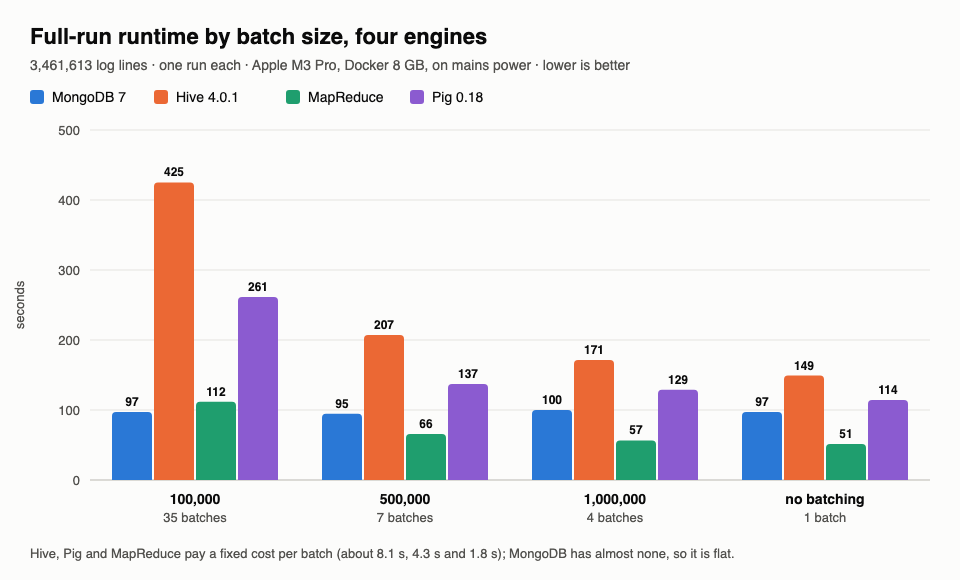
\includegraphics[width=\columnwidth]{benchmark_runtime.png}
\caption{Runtime by batch size; whiskers show min--max of 3 runs.}
\label{fig:bench}
\end{figure}

\section{Relational Reporting Schema}
PostgreSQL holds one schema, \code{etl} (Table~\ref{tab:schema}). Every result row carries
the pipeline, run ID, batch ID and execution time. A batch ID of 1 to $n$ marks that batch's
own results; \code{NULL} marks the whole-run result, and
\code{UNIQUE NULLS NOT DISTINCT} allows exactly one whole-run set per run. \code{CHECK}
constraints reject inconsistent data (valid plus malformed must equal the total; the error
rate must equal errors over total), and the average batch size is a generated column.

\begin{table}[t]
\caption{Tables in the PostgreSQL reporting schema}
\label{tab:schema}
\centering
\small
\begin{tabular}{@{}p{0.36\columnwidth}p{0.56\columnwidth}@{}}
\toprule
Table & Contents \\
\midrule
\code{etl\_run} & pipeline, batch size, status, runtime, counts, input hash \\
\code{etl\_batch} & batch ID, line range, record/valid/malformed counts, time \\
\code{query\_def} & Q1--Q3 names and definitions \\
\code{query\_execution} & per query and batch: rows, time, SHA-256 fingerprint \\
\code{q1\_daily\_traffic} & date, status, requests, bytes \\
\code{q2\_top\_resources} & path, requests, bytes, distinct hosts \\
\code{q3\_hourly\_errors} & date, hour, errors, total, rate, error hosts \\
\code{malformed\_record} & raw text of every malformed line \\
\bottomrule
\end{tabular}
\end{table}

The reporting module (\code{python -m etl report}) reads only views: \code{v\_run\_report}
and \code{v\_batch\_report} for metadata (pipeline, query names, runtime, batch IDs, batch
size, average batch size, per-query times), \code{v\_q1/q2/q3\_final} for results, and
\code{v\_pipeline\_comparison} for runtimes. It can also export the full report as HTML.

\section{Ensuring Equivalence Across Pipelines}
Equivalence is designed in and then verified:
\begin{enumerate}
\item \textbf{Same input and environment:} unchanged files, identical byte batches, pinned
Docker images.
\item \textbf{Same rules:} regexes, month map and output columns live in \code{contracts/};
engines load them rather than copying them. Q2 ties break by path in byte order; Q3 keeps
hours with zero errors.
\item \textbf{Answer key:} a test-only Python engine runs the same contracts and produced
\code{reference\_results.json}; it is hidden from the report.
\item \textbf{Fingerprints:} each query result gets a SHA-256 over its sorted rows (Q3's
floating-point rate excluded); the view \code{v\_equivalence} flags any disagreement.
\item \textbf{Row-by-row check:} \code{python -m etl.compare} joins two runs in PostgreSQL and
compares every row of every batch and the whole run (error rate within $10^{-12}$), and refuses
runs with different inputs or batch sizes.
\end{enumerate}
\textbf{Result.} Hive and MongoDB at $N=500{,}000$ agree on all 614 Q1, 160 Q2 and 2,744 Q3
rows across 7 batches plus the whole run, with identical malformed lines; all 18 benchmark
runs at three batch sizes share one fingerprint per query. A 16-test database suite and the
smoke test guard against regressions.

\section{Status and Next Steps}
Completed: contracts and schema, Docker environment, controller and loader, MongoDB and Hive
engines, equivalence checker, benchmarks and the reporting module. Phase~2 adds Pig and
MapReduce as two more implementations of the same engine interface, verified with the same
contracts, checker and benchmarks.

\begin{thebibliography}{1}
\bibitem{nasa} NASA Kennedy Space Center WWW server logs, Internet Traffic Archive.
\url{https://ita.ee.lbl.gov/html/contrib/NASA-HTTP.html}
\bibitem{mongo} MongoDB 7.0 Manual: Aggregation, \texttt{\$regexFind}, \texttt{\$group}, \texttt{\$merge}.
\bibitem{hive} Apache Hive 4.0 Language Manual: RegexSerDe, ORC, multi-table insert.
\bibitem{pg} PostgreSQL 15 Documentation: \texttt{COPY}, unique constraints, generated columns.
\end{thebibliography}

\end{document}
